\documentclass[10pt,]{article}
\usepackage{geometry}
\geometry{margin=2.5cm}
\usepackage{graphicx}
\usepackage{xcolor}

% Custom Premium Researcher Typography: Linux Libertine (automatically includes Biolinum)
\usepackage{libertine}

\usepackage{booktabs}
\usepackage{longtable}
\usepackage{float}
\usepackage{array}
\usepackage{caption}
\usepackage{titlesec}
\usepackage{fancyhdr}
\usepackage{url}
\usepackage{hyperref}
\usepackage{setspace} % Load setspace package for spacing environments

\newcommand{\logoUNL}{/home/erick-fcs/Capital_Workstation/capital-workstation-libs/src/ecs_quantitative/reporting/assets/logos/logo_unl.png}
\newcommand{\logoECONOMIA}{/home/erick-fcs/Capital_Workstation/capital-workstation-libs/src/ecs_quantitative/reporting/assets/logos/logo_economia.jpg}\newenvironment{referenciasAPA}{\setlength{\parindent}{-1.27cm}\setlength{\leftskip}{1.27cm}\setlength{\parskip}{6pt}}{\par}
\newcommand{\fuente}[1]{\vspace{-2pt}\noindent\small\textit{Nota.} #1}\makeatletter\@ifpackageloaded{caption}{}{\usepackage{caption}}\AtBeginDocument{%
\ifdefined\contentsname
  \renewcommand*\contentsname{Table of contents}
\else
  \newcommand\contentsname{Table of contents}
\fi
\ifdefined\listfigurename
  \renewcommand*\listfigurename{List of Figures}
\else
  \newcommand\listfigurename{List of Figures}
\fi
\ifdefined\listtablename
  \renewcommand*\listtablename{List of Tables}
\else
  \newcommand\listtablename{List of Tables}
\fi
\ifdefined\figurename
  \renewcommand*\figurename{Figure}
\else
  \newcommand\figurename{Figure}
\fi
\ifdefined\tablename
  \renewcommand*\tablename{Table}
\else
  \newcommand\tablename{Table}
\fi
}\@ifpackageloaded{float}{}{\usepackage{float}}
\floatstyle{ruled}
\@ifundefined{c@chapter}{\newfloat{codelisting}{h}{lop}}{\newfloat{codelisting}{h}{lop}[chapter]}
\floatname{codelisting}{Listing}\newcommand*\listoflistings{\listof{codelisting}{List of Listings}}\makeatother\makeatletter\makeatother\makeatletter\@ifpackageloaded{caption}{}{\usepackage{caption}}
\@ifpackageloaded{subcaption}{}{\usepackage{subcaption}}\makeatother

% Curated Academic Palette (Prussian Blue, Burgundy, Soft Charcoal)
\definecolor{primary}{HTML}{0A2540}    % Deep Prussian Blue
\definecolor{secondary}{HTML}{8D2B32}  % Sophisticated Deep Burgundy
\definecolor{darkgray}{HTML}{22252A}   % Rich Slate/Charcoal for body text

% Apply dark gray color to body text
\makeatletter
\newcommand{\globalcolor}[1]{%
  \color{#1}\global\let\default@color\current@color
}
\makeatother
\AtBeginDocument{\globalcolor{darkgray}}

% Section heading styles
\titleformat{\section}
  {\color{primary}\normalfont\Large\bfseries\sffamily}
  {\thesection}{1em}{}
\titleformat{\subsection}
  {\color{secondary}\normalfont\large\bfseries\sffamily}
  {\thesubsection}{1em}{}

\titlespacing*{\section}{0pt}{14pt}{6pt}
\titlespacing*{\subsection}{0pt}{10pt}{4pt}

% Caption styling
\DeclareCaptionFont{primarycolor}{\color{primary}}
\captionsetup[table]{name=Tabla, format=plain, labelsep=newline, justification=raggedright, singlelinecheck=false, labelfont={bf,primarycolor,normalsize}, textfont={it,normalsize}}
\captionsetup[figure]{name=Figura, format=plain, labelsep=newline, justification=raggedright, singlelinecheck=false, labelfont={bf,primarycolor,normalsize}, textfont={it,normalsize}}

% Header & Footer
\pagestyle{fancy}
\fancyhf{}
\fancyhead[L]{\sffamily\small\color{secondary}PROPUESTA DE POLÍTICA PÚBLICA}
\fancyhead[R]{\sffamily\small\color{secondary}EMPLEO ADECUADO Y FORMALIZACIÓN}
\fancyfoot[L]{\sffamily\small\color{gray}Erick Condoy Seraquive | Propuesta de Política Pública}
\fancyfoot[R]{\sffamily\small\color{gray}\thepage}
\renewcommand{\headrulewidth}{0.5pt}
\renewcommand{\headrule}{\hbox to\headwidth{\color{secondary}\leaders\hrule height \headrulewidth\hfill}}
\renewcommand{\footrulewidth}{0pt}

% Pull-quote environment
\newenvironment{pullquote}{%
  \vspace{10pt}
  \begin{center}
  \begin{minipage}{0.88\textwidth}
  \color{secondary} % Use Burgundy for highlights like pullquotes
  \hrule height 1pt
  \vspace{6pt}
  \centering\itshape\large
}{%
  \vspace{6pt}
  \hrule height 1pt
  \end{minipage}
  \end{center}
  \vspace{10pt}
}

\providecommand{\tightlist}{%
  \setlength{\itemsep}{0pt}\setlength{\parskip}{0pt}}

\begin{document}
\begin{center}
\sffamily
{\color{primary}\Huge\bfseries Propuesta de Política Pública: \\ Formalización Laboral y Estímulo al Empleo Adecuado en el Ecuador} \\
\vspace{1.5em}
{\color{darkgray}\large\bfseries Erick Condoy Seraquive} \\
\textit{Estudiante de Economía | UNL --- Investigación en Mercado Laboral y Política Pública} \\
\vspace{0.8em}
\sffamily\small Mayo de 2026
\end{center}

\begin{center}
\sffamily\small
\begin{tabular}{rl}
\textbf{Horizonte de Implementación:} & 18--24 meses (Fase Piloto en Cañar, Bolívar y Loja) \\
\textbf{Meta de Impacto Principal:} & Reducción de la informalidad laboral rural del 75.8\% al 65.0\% en 5 años \\
\end{tabular}
\end{center}
\vspace{1.2em}

\begin{center}
\begin{minipage}{0.9\textwidth}
\begin{spacing}{1.15}
\sffamily\small
\color{primary}
\textbf{Resumen Ejecutivo} ---
\textit{Ecuador registra un 3.7\% de desempleo y un 55.2\% de informalidad laboral. Esta paradoja no constituye una anomalía aislada, sino el síntoma de un mercado laboral atrapado entre la dolarización, el déficit fiscal y la ausencia de incentivos estructurales a la formalización. Esta propuesta diseña un programa de tres instrumentos operativos con base en evidencia cuantitativa regional (Chile, Colombia) y microdatos de la ENEMDU 2025 para revertir de manera progresiva esta tendencia estructural.}
\end{spacing}
\end{minipage}
\end{center}
\vspace{1.5em}

\section{Diagnóstico Estructural del Mercado Laboral
Ecuatoriano}\label{diagnuxf3stico-estructural-del-mercado-laboral-ecuatoriano}

El mercado laboral ecuatoriano presenta un bajo nivel de desempleo
abierto (\(3.7\%\) a nivel nacional, \(5.0\%\) urbano y \(1.4\%\) rural)
(INEC, 2025a), una cifra que enmascara una profunda precariedad
subyacente. Ante la ausencia de un sistema de protección social
universal de amplia cobertura, gran parte de la fuerza laboral se
inserta en actividades informales de baja productividad y bajos
salarios. A nivel nacional, el empleo adecuado alcanza apenas al
\(35.9\%\) de la población económicamente activa (PEA) (INEC, 2025a).

Esta problemática estructural exhibe agudas brechas territoriales y de
género: 1. \textbf{Brecha de Género}: El acceso al empleo adecuado se
sitúa en un \(41.4\%\) para los hombres, mientras que para las mujeres
desciende de manera crítica al \(28.4\%\) (INEC, 2025a), evidenciando
marcadas barreras de inserción. 2. \textbf{Brecha Territorial}: En las
zonas rurales, el empleo adecuado se desploma al \(19.4\%\). La
informalidad laboral en este ámbito constituye la norma de subsistencia,
afectando al \(75.8\%\) de la fuerza de trabajo en comparación con el
\(43.6\%\) registrado en áreas urbanas (INEC, 2025b). La Figura
\ref{fig:diagnostico_laboral} expone esta distribución estructural del
empleo en el país.

\begin{pullquote}
``En el sector rural del Ecuador, la informalidad laboral constituye la norma de subsistencia afectando al 75.8\% de la fuerza de trabajo, mientras el empleo adecuado se desploma a un alarmante 19.4\%.''
\end{pullquote}

\begin{figure}[H]
\centering
\caption{Polarización Estructural del Mercado Laboral Ecuatoriano}
\label{fig:diagnostico_laboral}
\vspace{2pt}
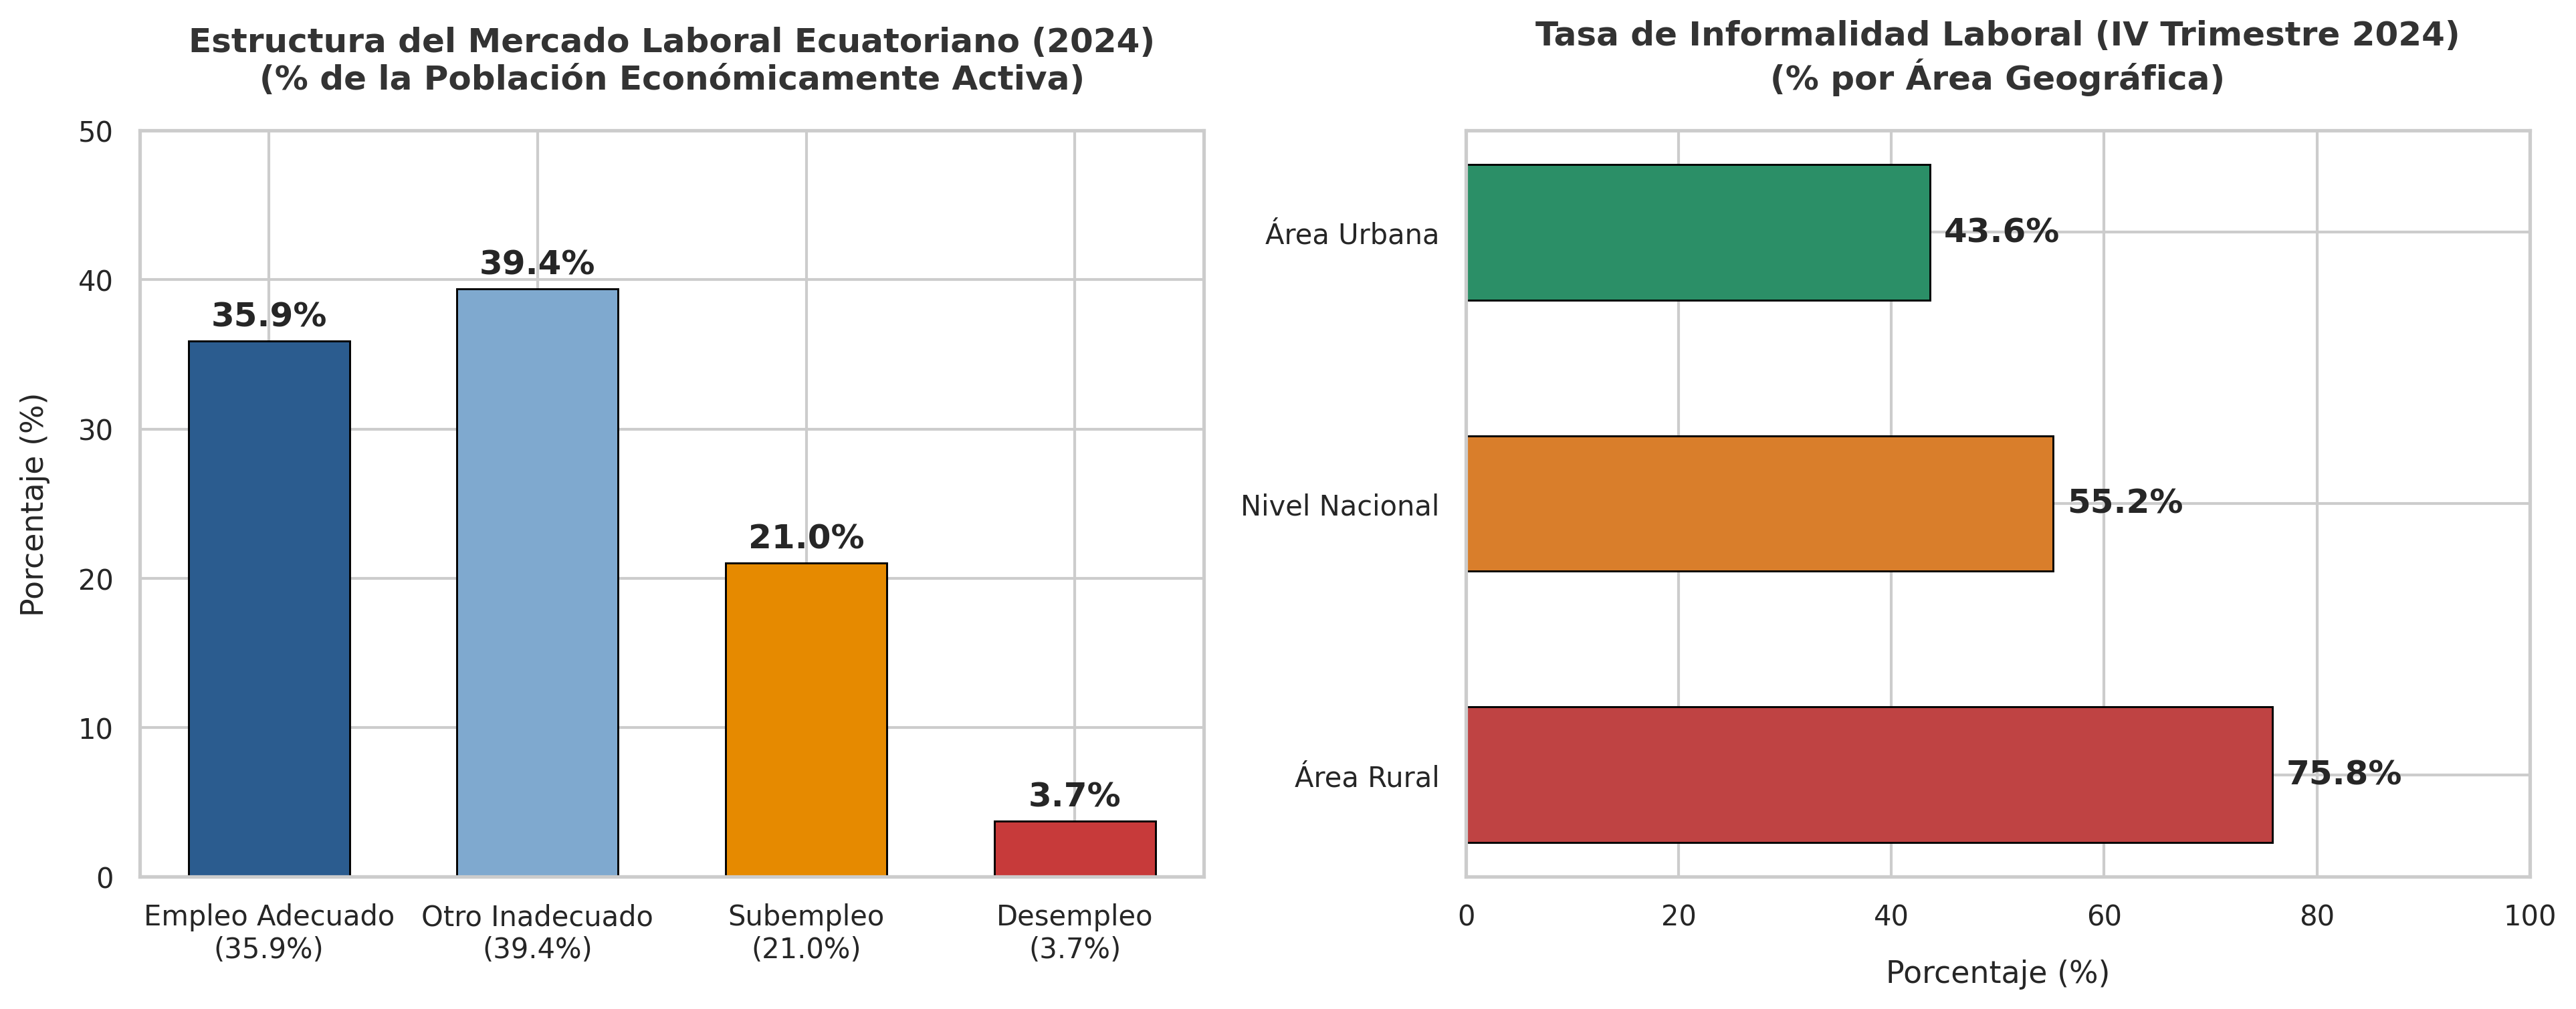
\includegraphics[width=0.95\textwidth]{assets/diagnostico_laboral.png}
\vspace{-2pt}
\fuente{Elaboración propia con base en boletines técnicos de la ENEMDU (INEC, 2025a, 2025b).}
\end{figure}

\section{Enfoque Teórico y Coherencia
Conceptual}\label{enfoque-teuxf3rico-y-coherencia-conceptual}

Bajo el esquema de dolarización y severa restricción de caja fiscal del
Ecuador, la imposibilidad de aplicar devaluaciones cambiarias o
monetizar déficits fiscales neutraliza los estímulos macroeconómicos
tradicionales de corto plazo. En este escenario, la persistencia de la
informalidad laboral rural responde a una marcada heterogeneidad
productiva y a barreras institucionales, no a desajustes cíclicos de
demanda (Weller, 2016; CEPAL, 2024). Por consiguiente, resolver esta
segmentación del mercado laboral exige una intervención microeconómica
bidireccional: políticas activas que eleven la productividad marginal
del trabajo mediante la capacitación técnica, y reformas de incentivos
específicos que reduzcan los costos no salariales de entrada a la
formalidad para las unidades productivas agrícolas y de servicios de
subsistencia.

\section{Diseño de Política Pública: Programa de Empleo Adecuado y
Formalización
Territorial}\label{diseuxf1o-de-poluxedtica-puxfablica-programa-de-empleo-adecuado-y-formalizaciuxf3n-territorial}

Se plantea el \textbf{``Programa de Empleo Adecuado y Formalización
Territorial para Mujeres y Jóvenes''}, con la meta de reducir la
informalidad rural del \(75.8\%\) al \(65.0\%\) en 5 años. Este objetivo
se calibra según los impactos de subsidios a la contratación en América
Latina (como el SENCE de Chile: \(+8.2\) pp de aumento en formalidad),
adaptados a las provincias del piloto (Cañar, Bolívar y Loja) mediante
elasticidades empleo-costo estimadas por el BID (Alaimo et al., 2015).
El programa opera bajo tres ejes:

\begin{enumerate}
\def\labelenumi{\arabic{enumi}.}
\tightlist
\item
  \textbf{Subsidio Temporal a la Seguridad Social}: Cofinanciamiento
  estatal del \(50\%\) de la aportación patronal al Instituto
  Ecuatoriano de Seguridad Social (IESS) por un lapso de 6 a 12 meses
  para la contratación neta de jóvenes (18 a 29 años) y mujeres,
  abaratando el costo laboral marginal inicial (SENCE, s.f.). Para
  mitigar el riesgo de deserción pos-subsidio, se incluye una cláusula
  de retención obligatoria de 6 meses y un diseño de evaluación de
  impacto con grupo de control en la fase piloto.
\item
  \textbf{Capacitación Técnica Focalizada}: Programas cortos de
  cualificación técnica diseñados según la demanda específica del tejido
  productivo local (agroindustria y servicios de digitalización
  comercial), mejorando los niveles de empleabilidad (J-PAL, s.f.; con
  incrementos promedio constatados del \(18\%\) en ingresos de mujeres
  jóvenes egresadas a los 3 años de su inserción).
\item
  \textbf{Monotributo Progresivo}: Régimen tributario y de aportes
  unificado y simplificado para microempresas que transiten hacia la
  regularización de su plantilla, aminorando las cargas administrativas
  de la formalización (Congreso de Colombia, 2010; estimulando la
  creación y regularización de más de 350,000 unidades productivas en su
  primer año de vigencia).
\end{enumerate}

\emph{Mecanismo de Transmisión}: Los incentivos directos reducen el
costo inicial de formalización para las MIPYMES, en tanto que la
capacitación técnica eleva de forma permanente la productividad marginal
del trabajador. Este diferencial compensa de manera orgánica el retiro
gradual del subsidio, consolidando puestos de empleo adecuado y formal a
largo plazo.

\emph{Sostenibilidad y Mitigación de Riesgos}: Para evitar prácticas
oportunistas de sustitución de personal, la asignación del subsidio está
condicionada a incrementos netos auditados en la plantilla total de la
empresa ante el IESS. La viabilidad presupuestaria del subsidio patronal
(estimado en el \(0.15\%\) del PIB para la fase piloto) se fundamenta en
un esquema mixto de cofinanciamiento: (i) la reasignación parcial del
margen fiscal generado por la optimización y focalización selectiva del
subsidio a combustibles de alto octanaje (Súper), medida que no afecta
al transporte público ni a los sectores populares de la PEA, y (ii) la
estructuración de un fondo de cofinanciamiento para la reactivación
laboral respaldado por líneas de crédito específicas de organismos
multilaterales de desarrollo.

\section{Matriz de Diseño de la
Propuesta}\label{matriz-de-diseuxf1o-de-la-propuesta}

La Tabla \ref{tbl:matriz} detalla la estructura operativa y lógica del
programa:

\begin{singlespace}
\begin{small}
\begin{longtable}{p{4.5cm} p{10.5cm}}
\caption{Matriz de diseño del Programa de Empleo Adecuado y Formalización Territorial} \label{tbl:matriz} \\
\toprule
\textbf{Componente de Diseño} & \textbf{Desarrollo Operativo de la Propuesta} \\ \midrule
\textbf{Problema laboral diagnosticado} & Alta informalidad y baja generación de empleo adecuado, con severas brechas en mujeres y el sector rural. \\ \addlinespace
\textbf{Datos de sustento} & Informalidad: $55.2\%$ nacional, $75.8\%$ rural. Empleo adecuado: $35.9\%$ nacional, $19.4\%$ rural, $28.4\%$ mujeres (INEC, 2025a, 2025b). \\ \addlinespace
\textbf{Población objetivo} & Jóvenes (18-29 años), mujeres, trabajadores rurales y microempresas informales en Cañar, Bolívar y Loja. \\ \addlinespace
\textbf{Política propuesta} & Programa de Empleo Adecuado y Formalización Territorial para Mujeres y Jóvenes. \\ \addlinespace
\textbf{Tipo de política} & Mixta (Política activa de empleo y reforma institucional). \\ \addlinespace
\textbf{Instrumento concreto} & Subsidio del $50\%$ a la aportación patronal del IESS (6-12 meses) para contratación neta; capacitación técnica; monotributo simplificado. \\ \addlinespace
\textbf{Mecanismo económico} & La reducción de costos iniciales de formalización y la elevación de productividad marginal estimulan la demanda de empleo formal en MIPYMES. \\ \addlinespace
\textbf{Indicador principal} & Variación neta de la tasa de empleo adecuado en la población beneficiaria (Meta: Reducción de $10.8$ puntos porcentuales de informalidad rural). \\ \addlinespace
\textbf{Indicadores secundarios} & Reducción de la tasa de informalidad rural; número de nuevas afiliaciones femeninas y jóvenes al IESS. \\ \addlinespace
\textbf{Riesgos identificados} & Oportunismo contractual (contratos temporales únicamente por subsidio), desplazamiento laboral y restricción de caja fiscal. \\ \addlinespace
\textbf{Medidas de mitigación} & Auditoría de adición neta de planillas; cláusulas de permanencia de 6 meses pos-subsidio; cofinanciamiento vía margen fiscal de combustibles y multilateral. \\ \bottomrule
\multicolumn{2}{@{}p{15cm}@{}}{\small\textit{Nota.} Elaboración propia con base en el marco conceptual de Weller (2016), Alaimo et al. (2015) y los indicadores del INEC (2025a, 2025b).}
\end{longtable}
\end{small}
\end{singlespace}

\section{Reflexión y Diálogo
Profesional}\label{reflexiuxf3n-y-diuxe1logo-profesional}

El diseño de políticas laborales en economías dolarizadas nos impone el
reto de innovar a través de incentivos institucionales y saltos de
productividad, dada la imposibilidad de devaluar la moneda o monetizar
déficits fiscales para sostener el empleo.

¿Qué ajustes o complementos consideras prioritarios para adaptar este
programa a la realidad de tu provincia o sector productivo? Quedo muy
atento a tus aportes en la sección de comentarios para enriquecer este
debate técnico y proponer soluciones aplicables a nuestro contexto.

\noindent \textbf{Contacto Profesional y Redes:}

\begin{itemize}
\tightlist
\item
  \textbf{LinkedIn:}
  \href{https://www.linkedin.com/in/erick-fcs-370925394/}{linkedin.com/in/erick-fcs-370925394}
\item
  \textbf{GitHub/Portafolio:}
  \href{https://github.com/EryckFCS}{github.com/EryckFCS}
\item
  \textbf{E-mail:}
  \href{mailto:erick.condoy@unl.edu.ec}{erick.condoy@unl.edu.ec}
\end{itemize}

\section{Referencias}\label{referencias}

\begin{referenciasAPA}
Alaimo, V., Bosch, M., Kaplan, D. S., Pagés, C., \& Ripani, L. (2015). \textit{Empleos para crecer: Cómo aumentar la productividad y fomentar la formalidad en América Latina}. Banco Interamericano de Desarrollo. \url{https://publications.iadb.org/es/empleos-para-crecer-como-aumentar-la-productividad-y-fomentar-la-formalidad-en-america-latina}

Comisión Económica para América Latina y el Caribe [CEPAL]. (2024). \textit{Panorama Social de América Latina y el Caribe 2024: Desafíos de la protección social y la informalidad laboral}. Santiago de Chile: CEPAL. \url{https://www.cepal.org/es/publicaciones/panorama-social-america-latina-caribe-2024}

Congreso de Colombia. (2010). \textit{Ley 1429 de 2010: Ley de Formalización y Generación de Empleo}. Función Pública de Colombia. \url{https://www.funcionpublica.gov.co/eva/gestornormativo/norma.php?i=39430}

Instituto Nacional de Estadística y Censos [INEC]. (2025a). \textit{Encuesta Nacional de Empleo, Desempleo y Subempleo (ENEMDU): Boletín técnico anual enero-diciembre 2024}. Quito: INEC. \url{https://www.ecuadorencifras.gob.ec/documentos/web-inec/EMPLEO/2024/anual/Boletin_tecnico_anual_enero-diciembre_2024.pdf}

Instituto Nacional de Estadística y Censos [INEC]. (2025b). \textit{Encuesta Nacional de Empleo, Desempleo y Subempleo (ENEMDU): Indicadores laborales IV trimestre 2024}. Quito: INEC. \url{https://www.ecuadorencifras.gob.ec/documentos/web-inec/EMPLEO/2024/Trimestre_IV/2024_IV_Trimestre_Mercado_Laboral.pdf}

J-PAL. (s.f.). \textit{Vocational training for disadvantaged youth in Colombia}. Abdul Latif Jameel Poverty Action Lab. \url{https://www.povertyactionlab.org/evaluation/vocational-training-disadvantaged-youth-colombia}

Servicio Nacional de Capacitación y Empleo [SENCE]. (s.f.). \textit{Subsidio al Empleo Joven}. Gobierno de Chile. \url{https://www.sence.gob.cl/personas/subsidio-al-empleo-joven}

Weller, J. (Ed.). (2016). \textit{Jóvenes y empleo en América Latina: desafíos y perspectivas}. Santiago de Chile: Comisión Económica para América Latina y el Caribe (CEPAL). \url{https://www.cepal.org/es/publicaciones/40188-jovenes-empleo-america-latina-desafios-perspectivas}
\end{referenciasAPA}
\end{document}
